% RQ1 Results: Participation Dynamics

\subsection{Overview}

We present results from \experimentruns{} simulation runs across two experiments investigating participation dynamics. Table~\ref{tab:rq1-overview} summarizes key findings.

\begin{table}[htbp]
\centering
\caption{RQ1 Results Overview}
\label{tab:rq1-overview}
\begin{tabular}{lcc}
\toprule
Metric & Exp 01 (Calibration) & Exp 03 (Quorum) \\
\midrule
Configurations & 9 & 10 \\
Runs per config & 30 & 15 \\
Total runs & 270 & 150 \\
\bottomrule
\end{tabular}
\end{table}

\subsection{Experiment 01: Participation Calibration}

\subsubsection{Turnout vs. Participation Targets}

\begin{figure}[htbp]
    \centering
    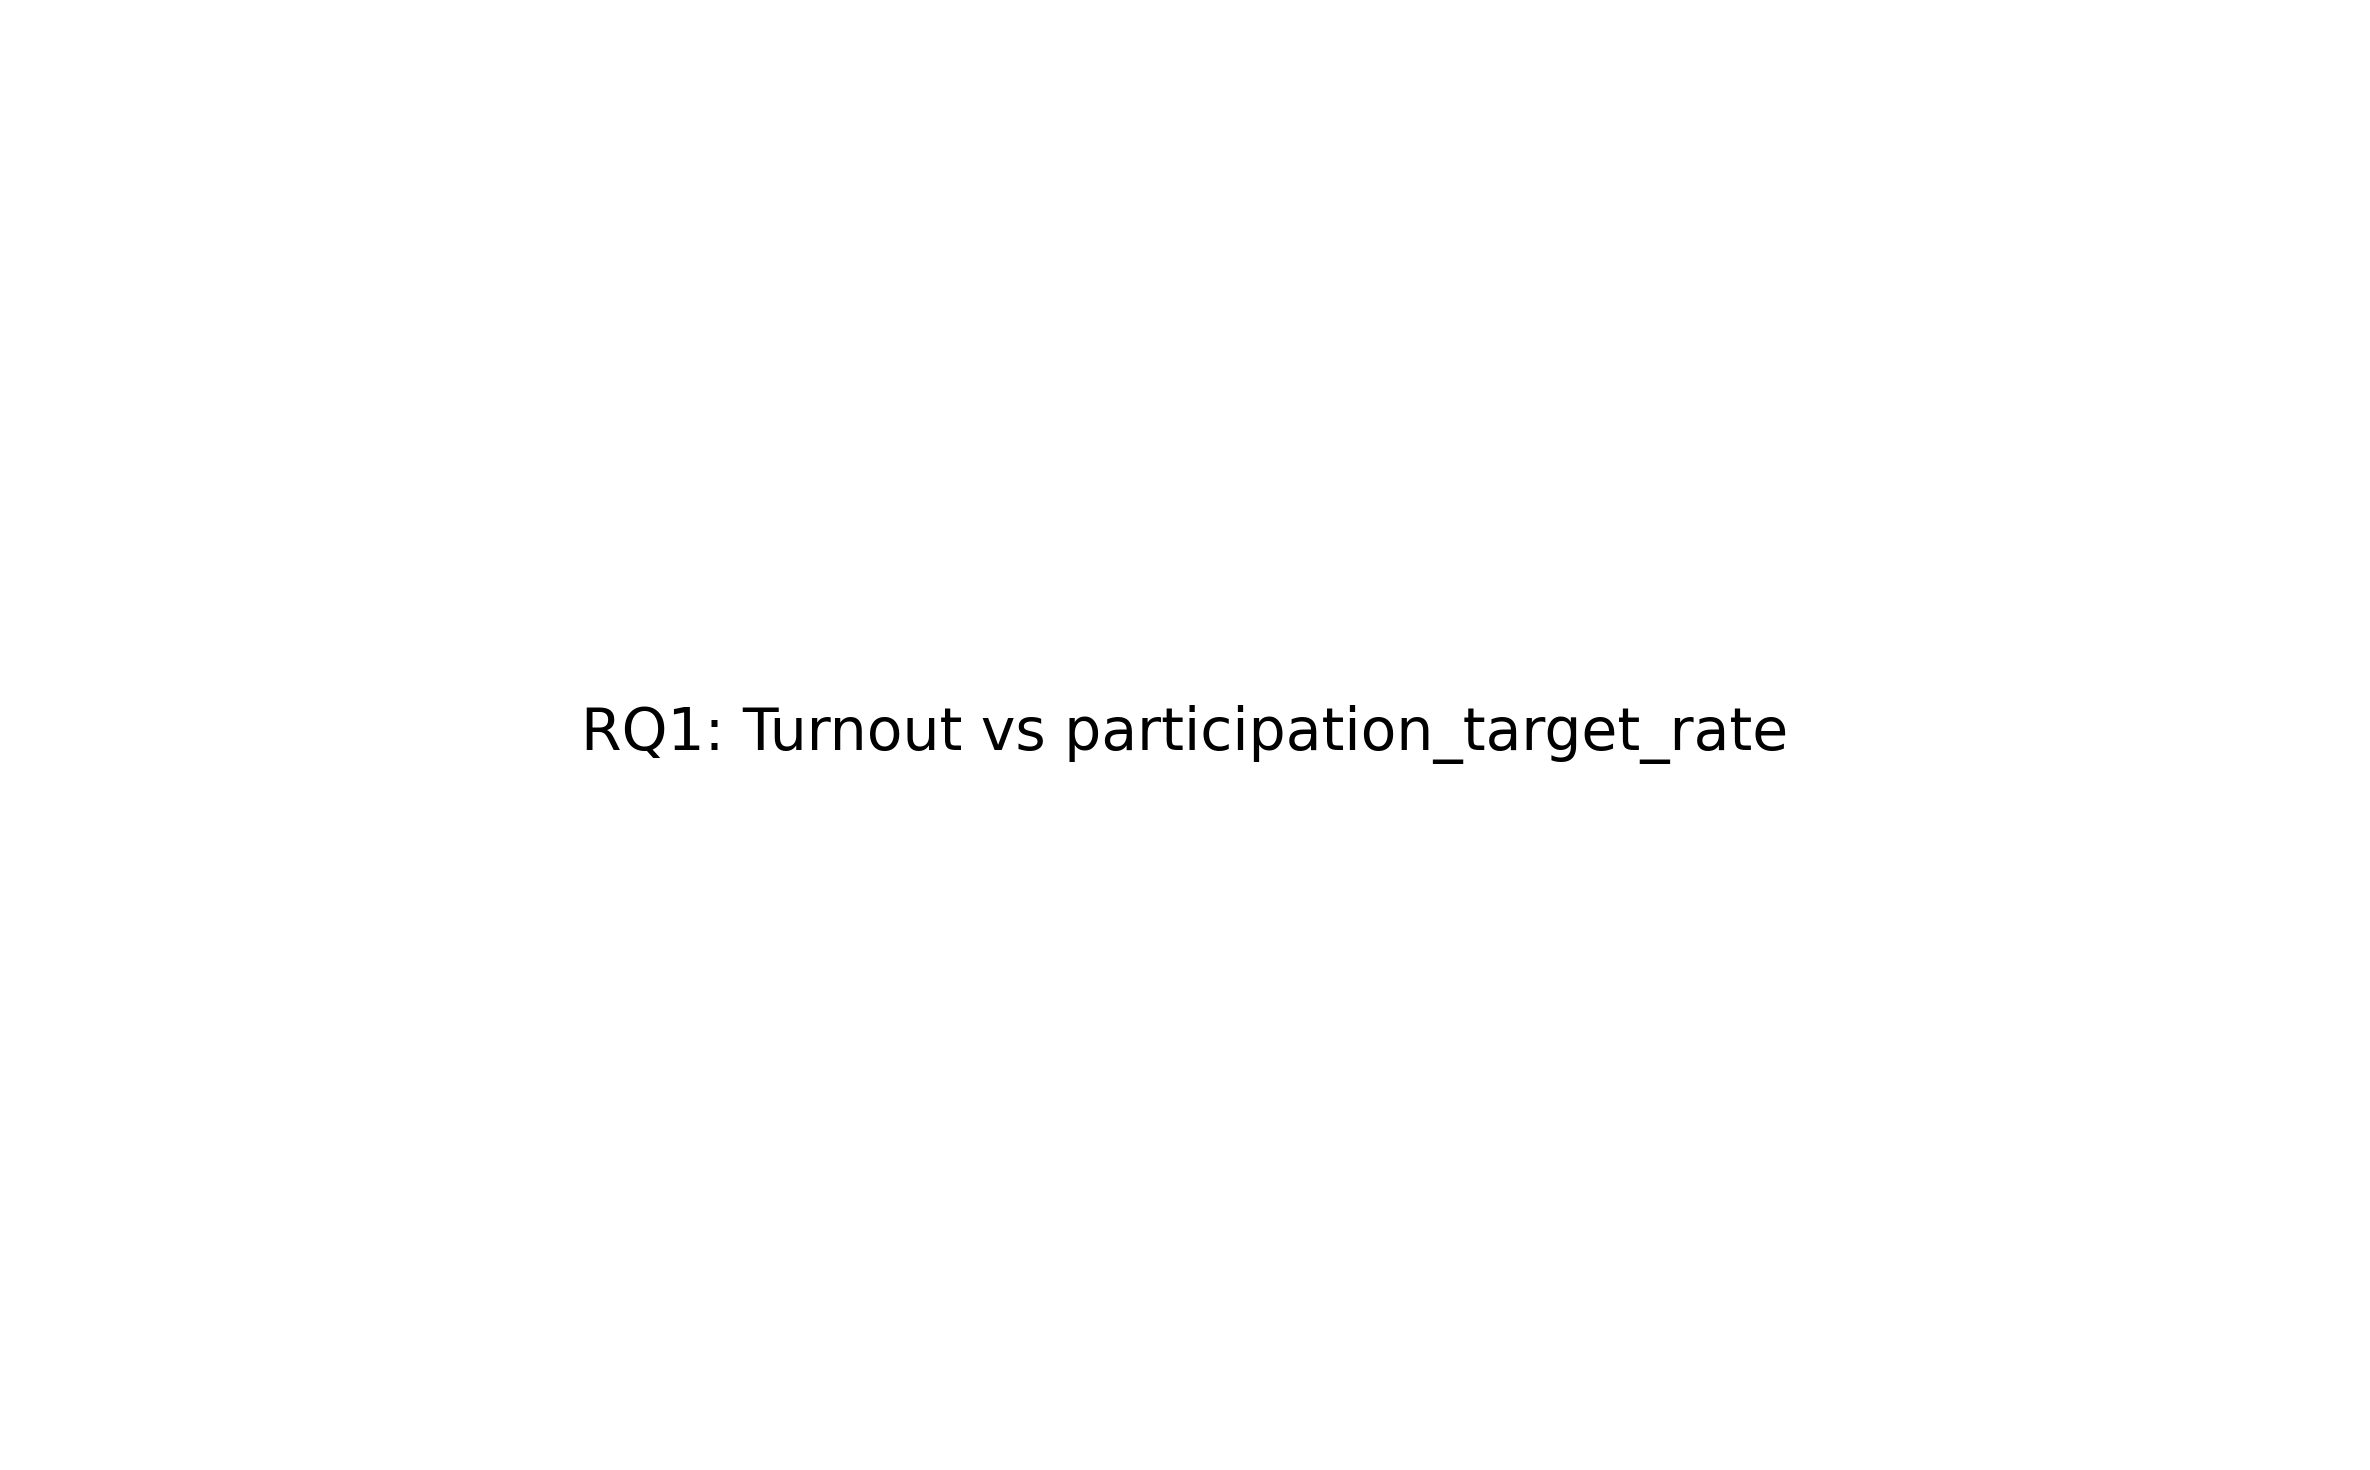
\includegraphics[width=0.8\textwidth]{../figures/rq1_turnout}
    \caption{Average turnout as a function of participation target rate. Error bars show 95\% CI. Higher targets do not proportionally increase turnout; diminishing returns are evident above 15\%.}
    \label{fig:rq1-turnout}
\end{figure}

\begin{table}[htbp]
\centering
\caption{Turnout by participation target (mean $\pm$ std)}
\label{tab:rq1-turnout}
\begin{tabular}{lccc}
\toprule
Target Rate & Turnout & Quorum Rate & 95\% CI \\
\midrule
\pl{5\%} & \pl{--} & \pl{--} & \pl{--} \\
\pl{15\%} & \pl{--} & \pl{--} & \pl{--} \\
\pl{30\%} & \pl{--} & \pl{--} & \pl{--} \\
\bottomrule
\end{tabular}
\end{table}

\subsubsection{Voter Retention}

\begin{figure}[htbp]
    \centering
    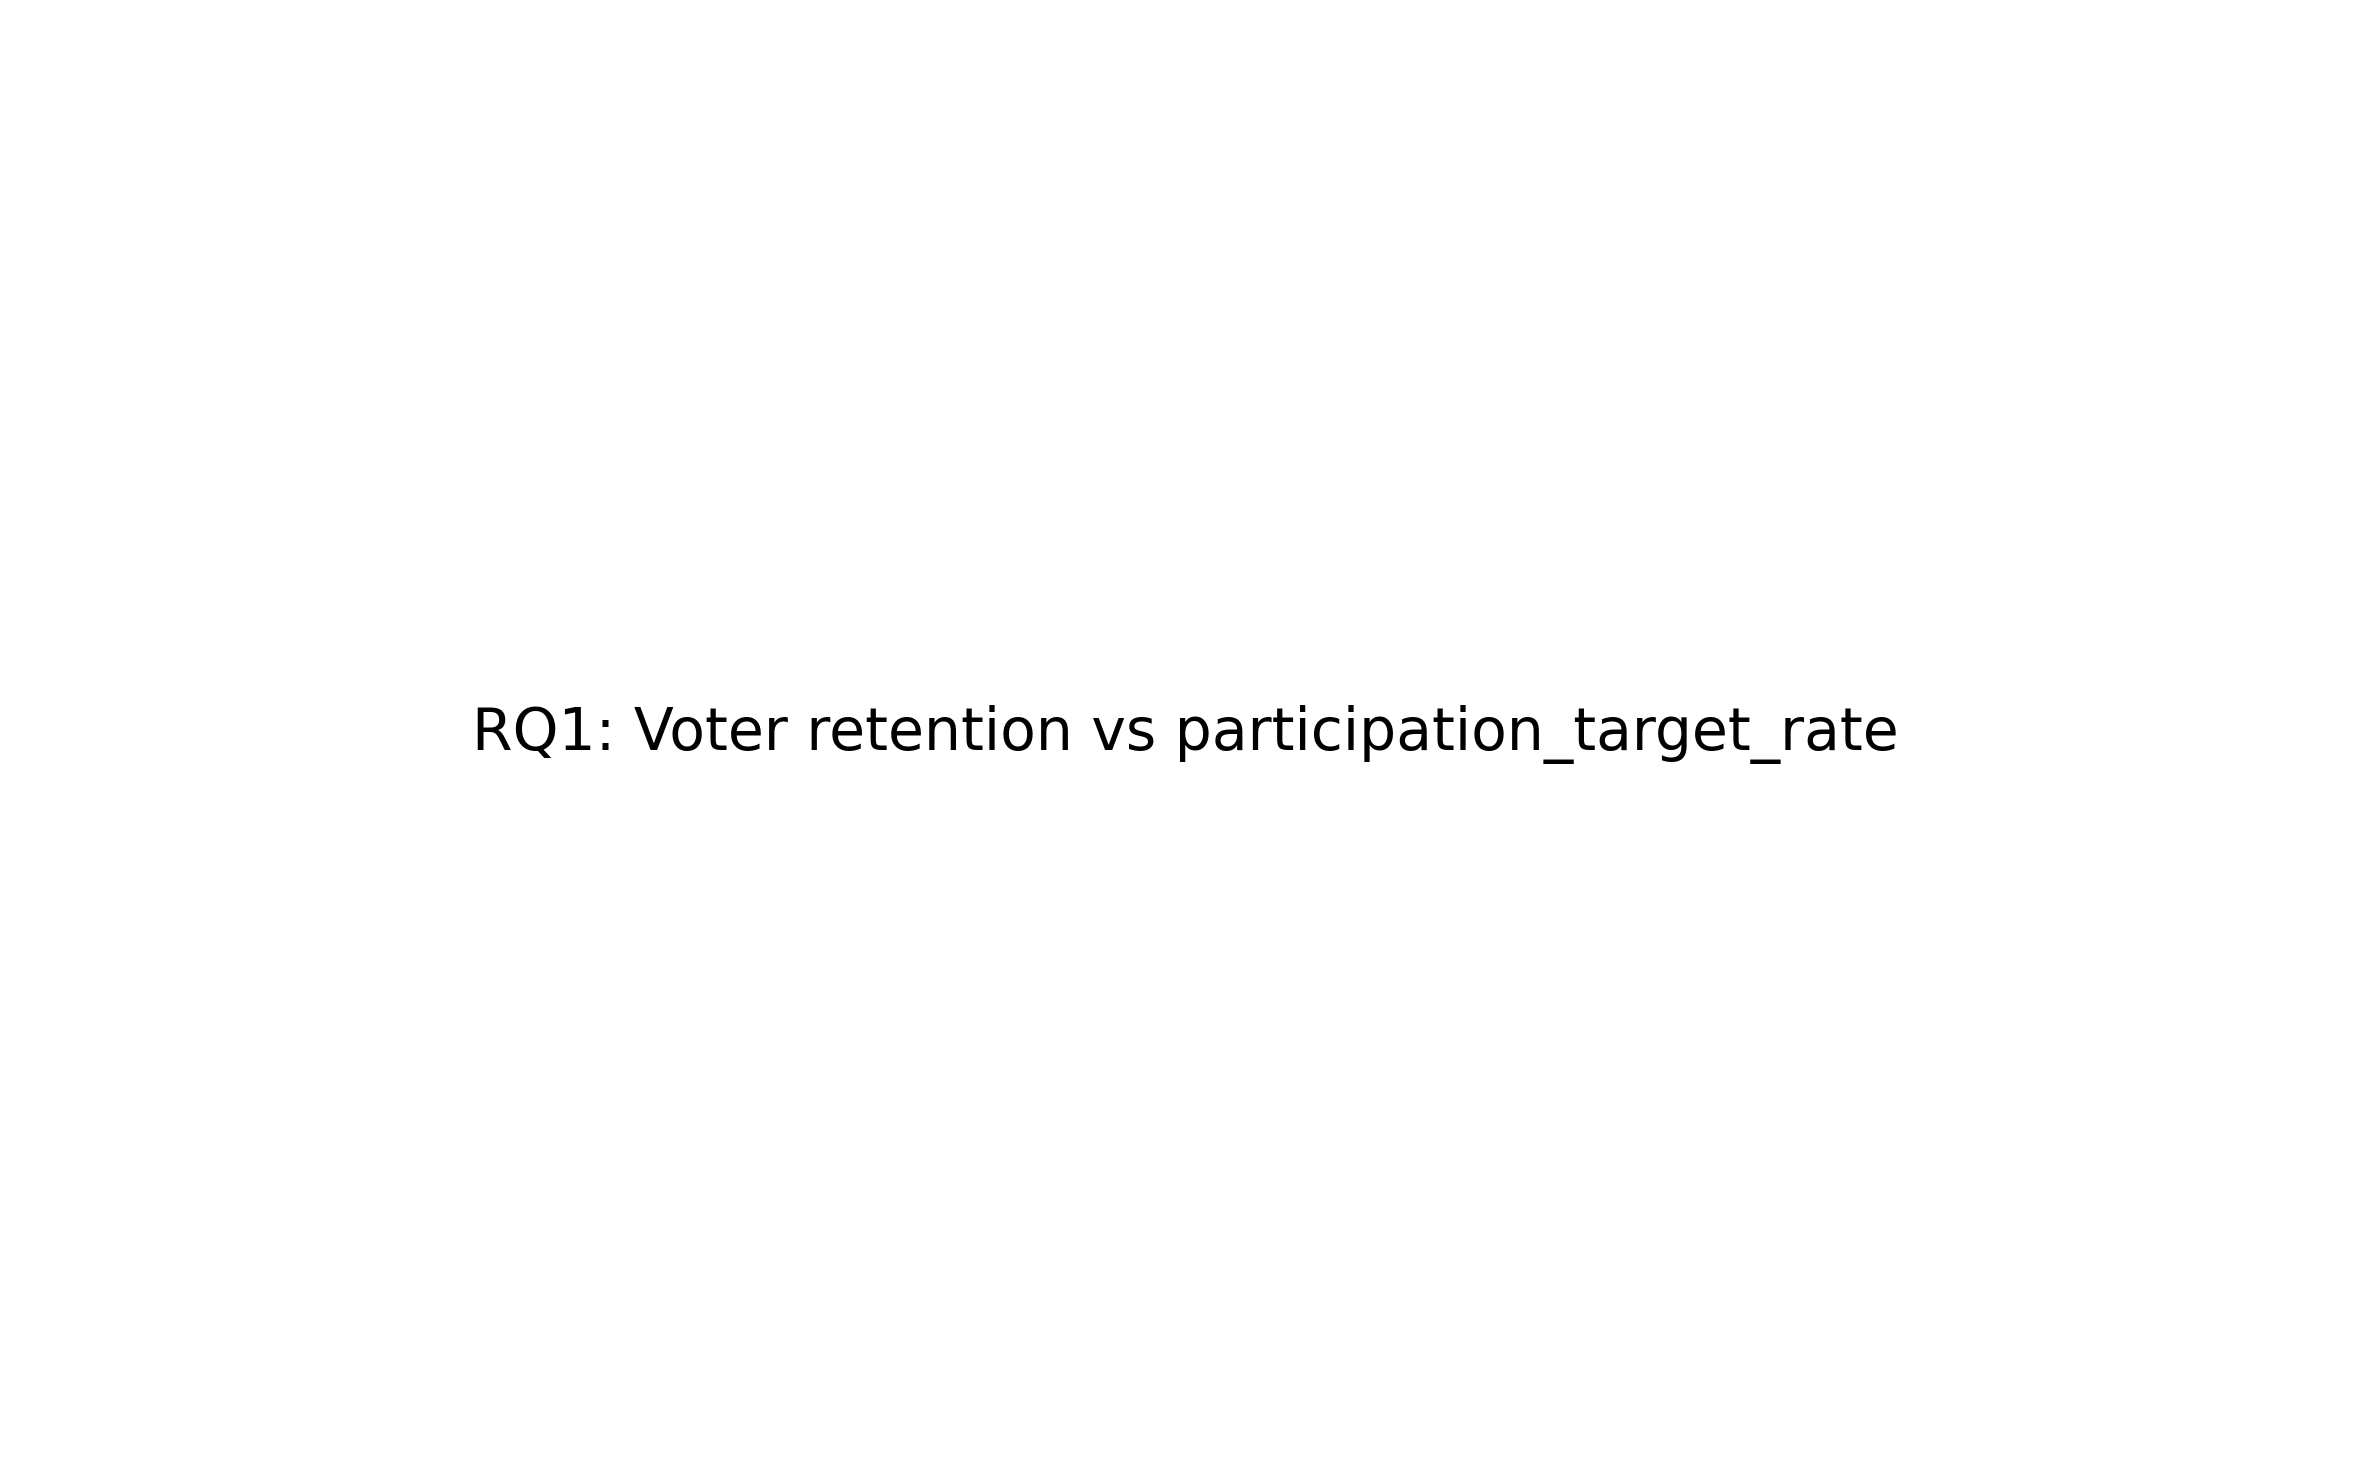
\includegraphics[width=0.8\textwidth]{../figures/rq1_retention}
    \caption{Voter retention (fraction of initially-active voters still participating at simulation end) decreases with higher participation targets, indicating unsustainable expectations lead to burnout.}
    \label{fig:rq1-retention}
\end{figure}

\begin{table}[htbp]
\centering
\caption{Retention and fatigue by target rate}
\label{tab:rq1-retention}
\begin{tabular}{lccc}
\toprule
Target Rate & Retention & Final Fatigue & Turnout Decay Rate \\
\midrule
\pl{5\%} & \pl{--} & \pl{--} & \pl{--} \\
\pl{15\%} & \pl{--} & \pl{--} & \pl{--} \\
\pl{30\%} & \pl{--} & \pl{--} & \pl{--} \\
\bottomrule
\end{tabular}
\end{table}

\subsubsection{Incentive Effects}

Stronger incentives partially compensate for aggressive targets:

\begin{table}[htbp]
\centering
\caption{Interaction of target rate and incentive strength}
\label{tab:rq1-interaction}
\begin{tabular}{lcccc}
\toprule
 & \multicolumn{3}{c}{Incentive Multiplier} \\
\cmidrule(lr){2-4}
Target & 0.5x & 1.0x & 2.0x \\
\midrule
\pl{5\%} & \pl{--} & \pl{--} & \pl{--} \\
\pl{15\%} & \pl{--} & \pl{--} & \pl{--} \\
\pl{30\%} & \pl{--} & \pl{--} & \pl{--} \\
\bottomrule
\end{tabular}
\end{table}

\subsection{Experiment 03: Quorum Sensitivity}

\subsubsection{Quorum-Pass Rate Curve}

\begin{figure}[htbp]
    \centering
    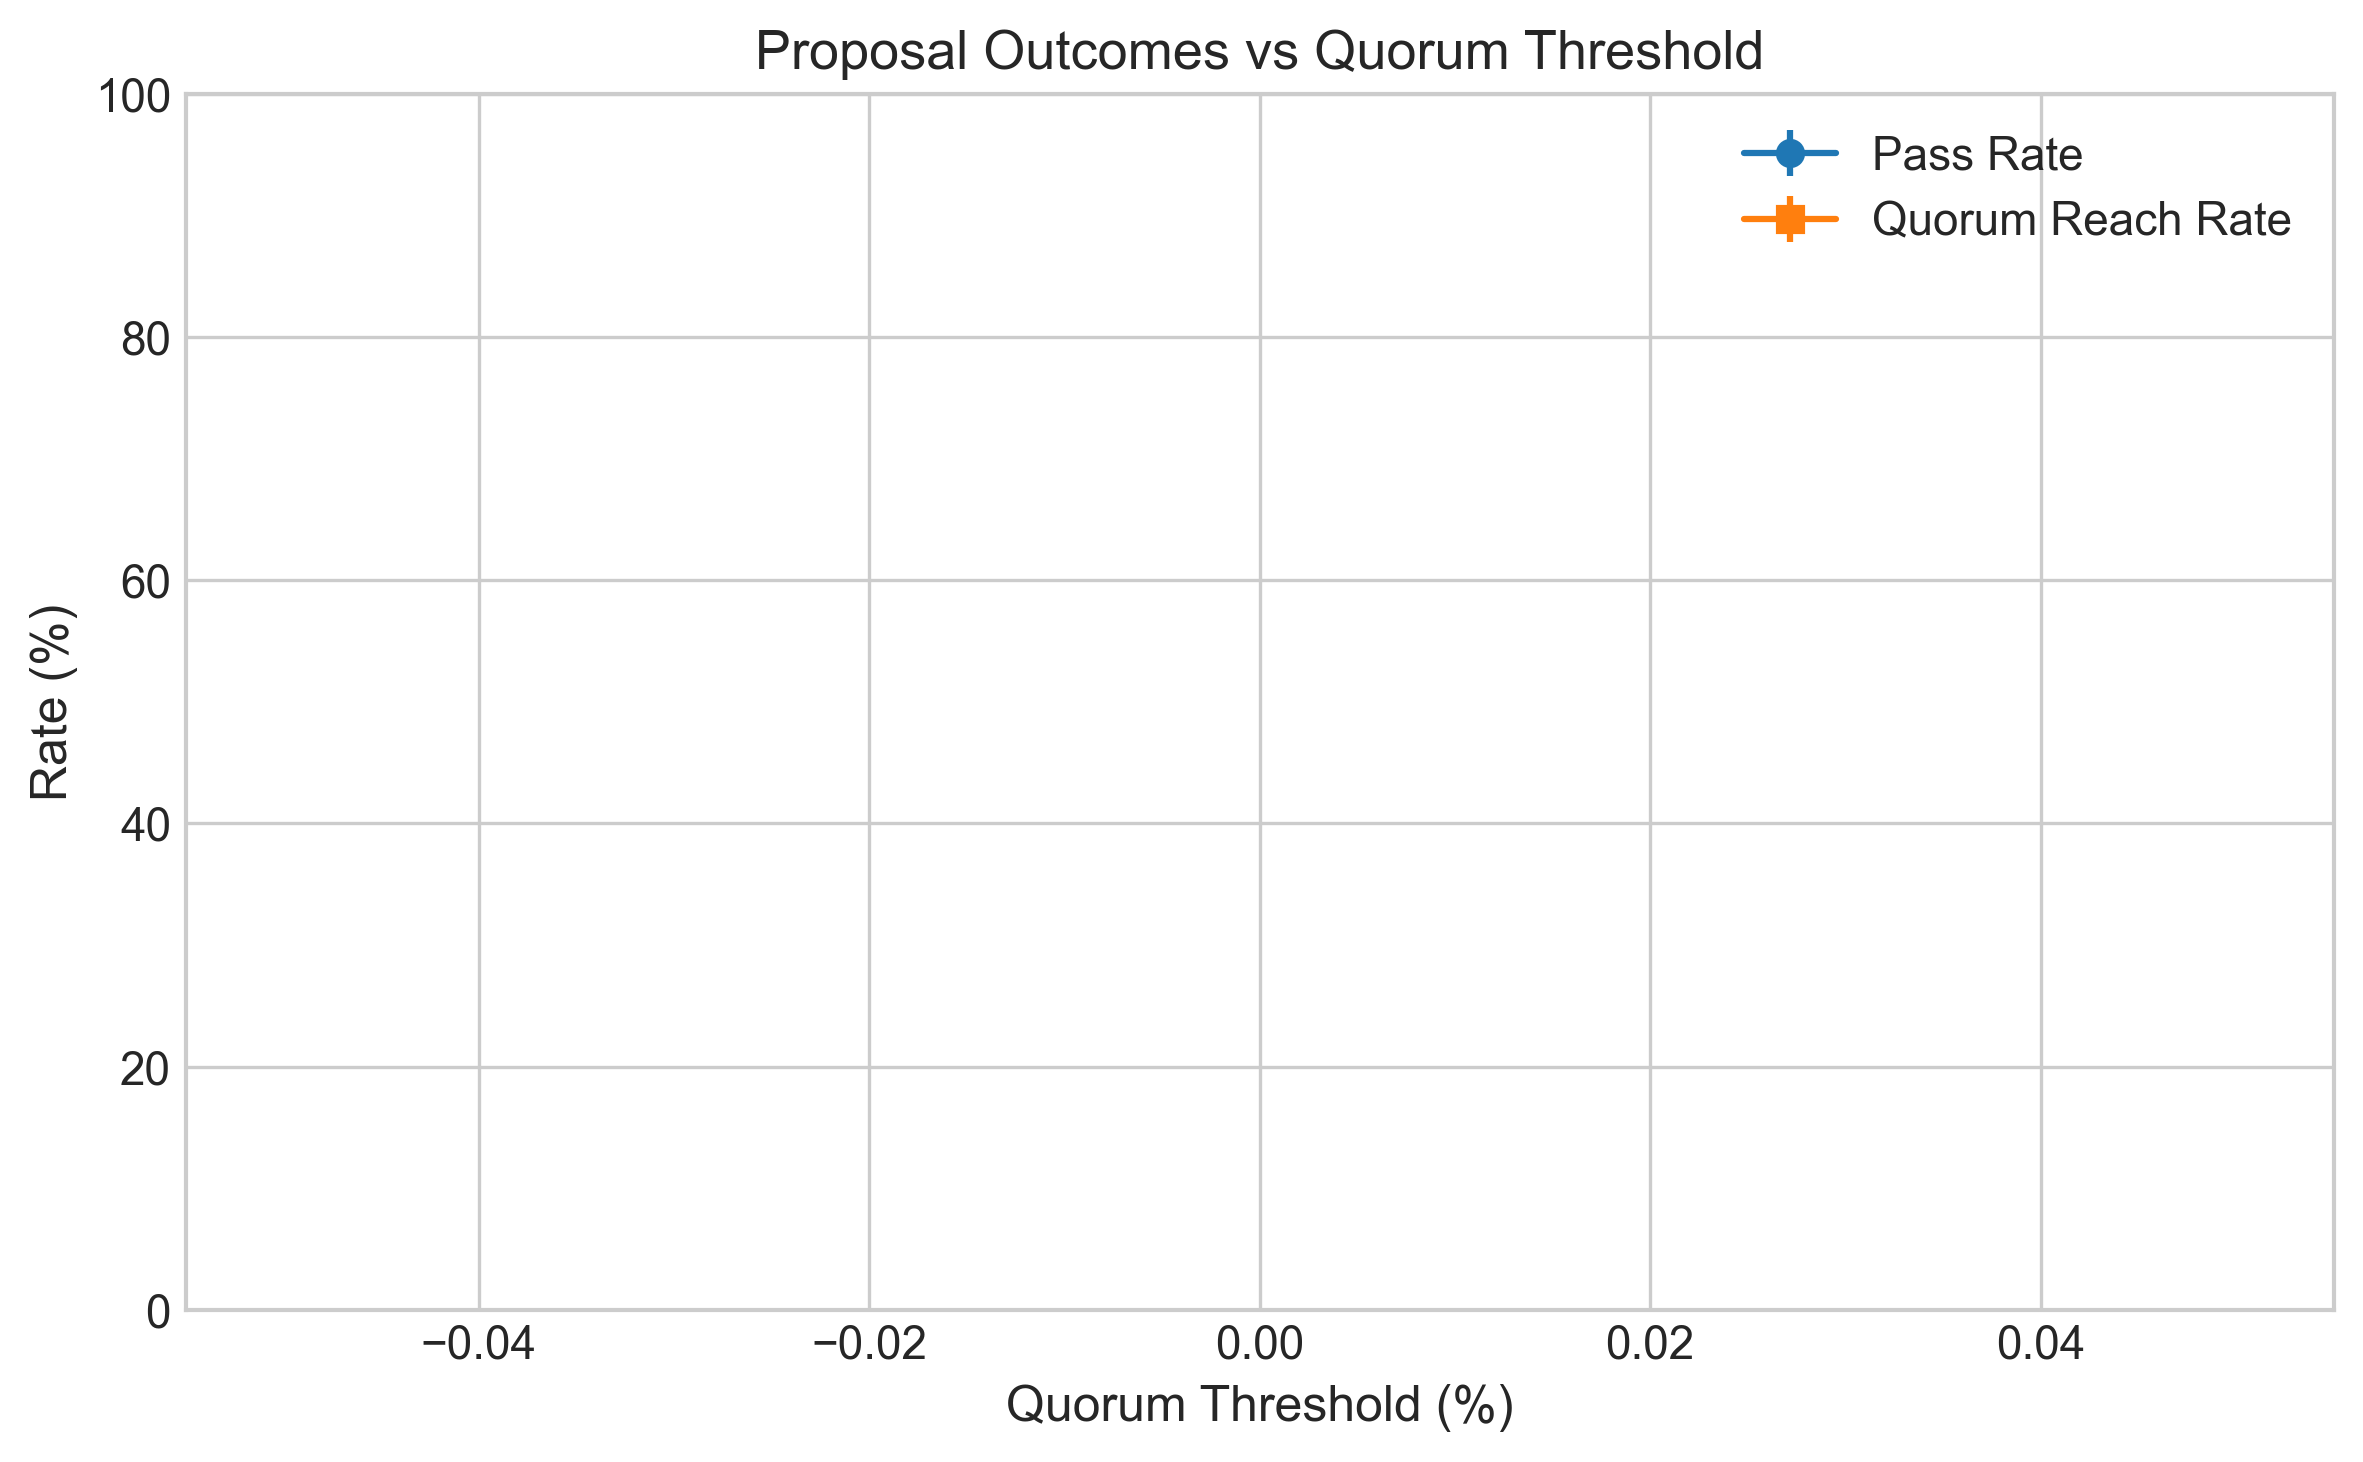
\includegraphics[width=0.8\textwidth]{../figures/rq1_quorum_curve}
    \caption{Proposal pass rate as a function of quorum threshold. The relationship is non-linear: pass rate remains high below 5\% quorum, then drops sharply. The inflection point suggests an optimal threshold around 4-5\%.}
    \label{fig:rq1-quorum-curve}
\end{figure}

\begin{table}[htbp]
\centering
\caption{Governance outcomes by quorum threshold}
\label{tab:rq1-quorum}
\begin{tabular}{lcccc}
\toprule
Quorum & Pass Rate & Quorum Failure & Avg Turnout & 95\% CI \\
\midrule
\pl{1\%} & \pl{--} & \pl{--} & \pl{--} & \pl{--} \\
\pl{2\%} & \pl{--} & \pl{--} & \pl{--} & \pl{--} \\
\pl{3\%} & \pl{--} & \pl{--} & \pl{--} & \pl{--} \\
\pl{4\%} & \pl{--} & \pl{--} & \pl{--} & \pl{--} \\
\pl{5\%} & \pl{--} & \pl{--} & \pl{--} & \pl{--} \\
\pl{6\%} & \pl{--} & \pl{--} & \pl{--} & \pl{--} \\
\pl{7\%} & \pl{--} & \pl{--} & \pl{--} & \pl{--} \\
\pl{8\%} & \pl{--} & \pl{--} & \pl{--} & \pl{--} \\
\pl{9\%} & \pl{--} & \pl{--} & \pl{--} & \pl{--} \\
\pl{10\%} & \pl{--} & \pl{--} & \pl{--} & \pl{--} \\
\bottomrule
\end{tabular}
\end{table}

\subsubsection{Fatigue Under High Quorum}

High quorum requirements increase fatigue as agents strain to meet thresholds:

\begin{figure}[htbp]
    \centering
    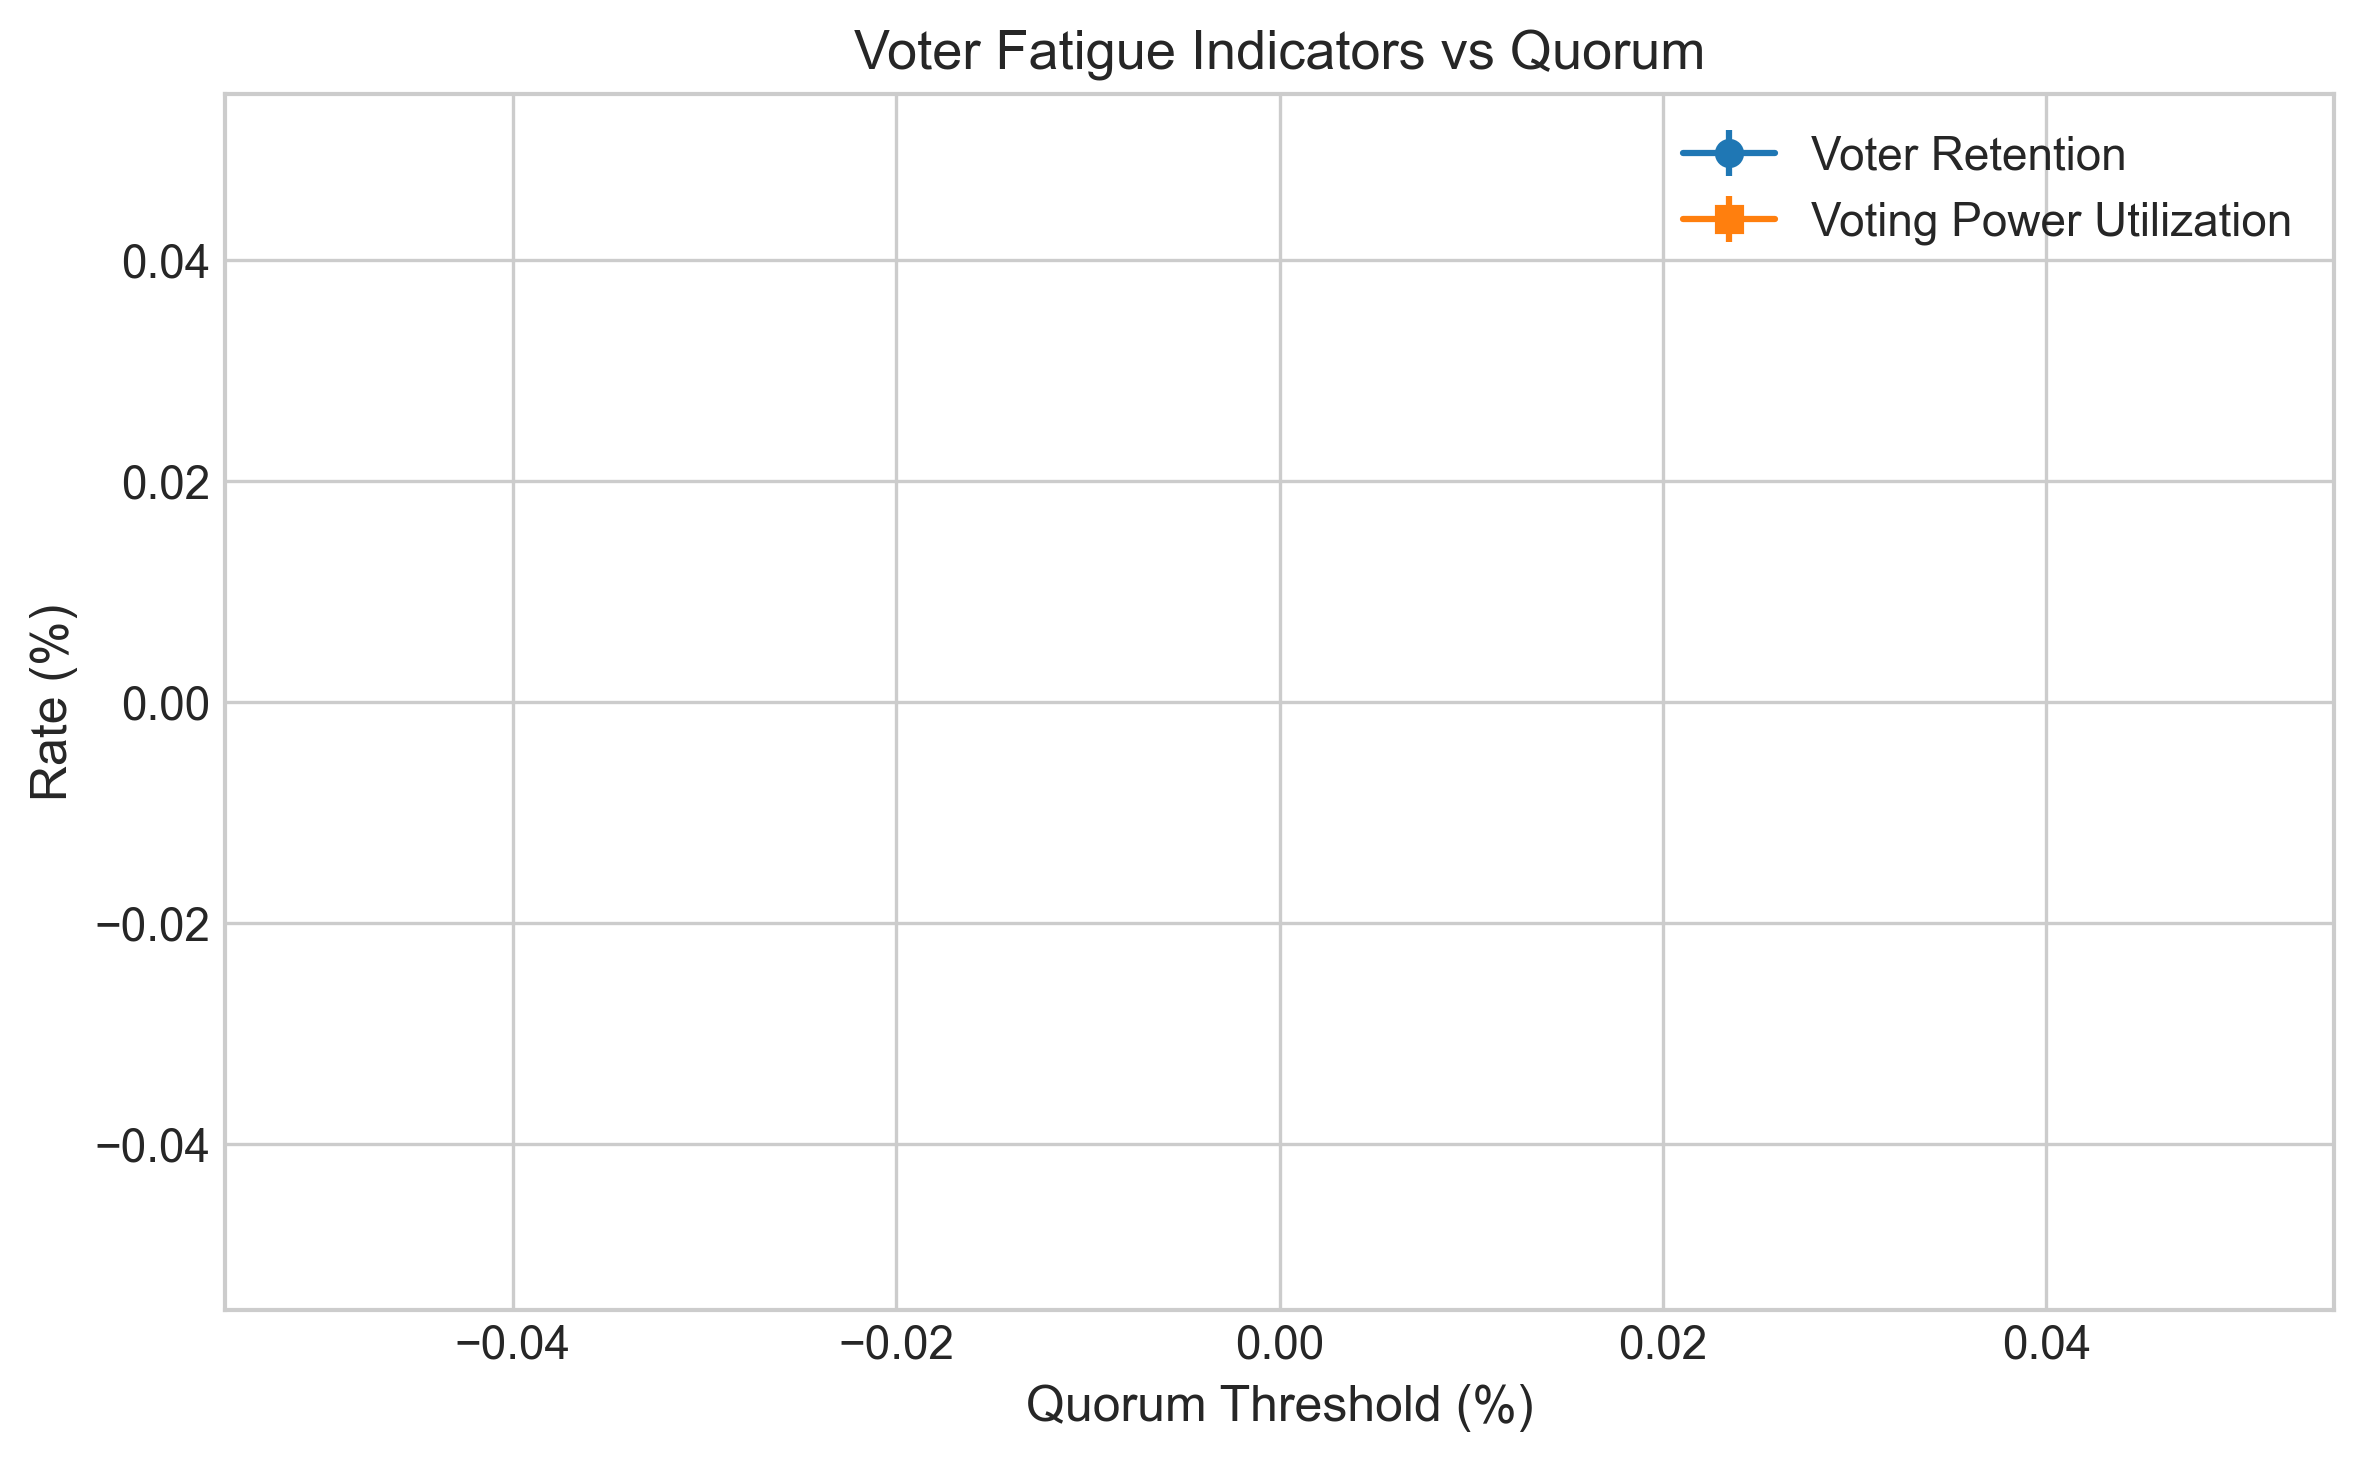
\includegraphics[width=0.8\textwidth]{../figures/rq1_fatigue_quorum}
    \caption{Mean fatigue at simulation end by quorum threshold. Higher quorums correlate with greater fatigue accumulation, suggesting governance strain.}
    \label{fig:rq1-fatigue-quorum}
\end{figure}

\subsection{Hypothesis Evaluation}

\begin{table}[htbp]
\centering
\caption{Hypothesis testing results}
\label{tab:rq1-hypotheses}
\begin{tabular}{llcc}
\toprule
Hypothesis & Test & $p$-value & Result \\
\midrule
H1.1: Higher targets $\rightarrow$ lower quorum achievement & ANOVA & \pl{--} & \pl{TBD} \\
H1.2: Incentives compensate for aggressive targets & Interaction & \pl{--} & \pl{TBD} \\
H1.3: High targets reduce retention & Regression & \pl{--} & \pl{TBD} \\
H3.1: Quorum-pass rate is non-linear & Polynomial fit & \pl{--} & \pl{TBD} \\
H3.2: Optimal quorum exists & Threshold analysis & \pl{--} & \pl{TBD} \\
H3.3: High quorum causes fatigue & Correlation & \pl{--} & \pl{TBD} \\
\bottomrule
\end{tabular}
\end{table}

\subsection{Key Findings}

\begin{enumerate}
    \item \textbf{Diminishing returns on targets}: Participation targets above 15\% yield rapidly diminishing turnout improvements while accelerating fatigue

    \item \textbf{Non-linear quorum curve}: The quorum-pass rate relationship shows a clear inflection point, suggesting natural ``governance capacity'' limits

    \item \textbf{Fatigue as binding constraint}: Long-term governance health is bounded by fatigue dynamics, not just instantaneous participation propensity

    \item \textbf{Incentive-target interaction}: Incentives can shift the curve but cannot overcome fundamental capacity constraints
\end{enumerate}
